\documentclass[letterpaper,twocolumn,10pt]{article}
\usepackage{usenix,epsfig,endnotes,color,cite,graphicx}% to put in axodraw
   % pictures, use colour in the document, put your citations as [1-4]
   % rather than [1,2,3,4] (it looks nicer, and the extended LaTeX2e
   % graphics package. 
\usepackage{latexsym,amssymb,epsf} % don't remember if these are
   % needed, but their inclusion can't do any damage
\usepackage{alltt}
\usepackage{graphicx}
\date{}
\begin{document}
\author{Ronald G. Minnich%
\thanks{\protect
\includegraphics[height=0.3in]{thunderchicken}%
}%
\thanks{Sandia is a multiprogram laboratory operated by Sandia Corporation, a Lockheed Martin Company, for the United States Department of Energy’s National Nuclear Security Administration under contract DE­AC04­94AL85000. SAND- 2009-5156C.}  
and John Floren\thanks{Sandia National Labs} 
and Eric Van Hensbergen\thanks{IBM} 
\\ 
and Jim McKie
\thanks{Bell Laboratories, Murray Hill, NJ, USA }
and Charles Forsyth
\thanks{Vita Nuova, Ldt.} and Roger Pearce\thanks{Lawrence Livermore National Laboratory}
}
%\institute{Ronald G. Minnich \at Sandia National Labs, Livermore, CA, 94550,
%    USA\\Tel.: 925-294-4713 %
%\email{rminnich@sandia.gov}  }

\title{\Large \bf Operating systems specializations: a technique to improve network  throughput for high performance computing}
\maketitle
\thispagestyle{empty}
\pagestyle{empty}
\subsection*{Abstract}
This paper explores the use of operating systems modifications, which we call {\em specializations}, as a technique for improving IO throughput in High Performance Computing (HPC) systems. 
These specializations are the software analog of the specializations implemented in chips such as the Power PC 4xx series used in the Blue Gene supercomputer. A 
specialization adds functionality that is not needed in a general purpose product, yet is essential to the correct operation of a special purpose product. It has  little use 
outside the HPC domain; its presence is the difference between success and failure in the HPC domain. 

In the Blue Gene hardware, a significant fraction of the floor plan is dedicated to special purpose subsystems. Conversely, our specializations are very small and simple, but have a dramatic impact on performance. 
They include: 
\begin{itemize}
\item Support for process-private system calls and currying for devices that require it
\item A bypass path in the system call that implements low latency access to a network driver
\item A hybrid process model in which certain distinguished processes share the heap (bss) segment with virtual-equal-physical addressing, allowing common memory addresses in programs, the kernel, and interrupt handlers
\item Support for {\em active messages} and {\em one-sided messaging} in the interrupt handler of a network driver
\end{itemize}

We have implemented and measured these changes using IBM Blue Gene supercomputers running under the Plan~9 research operating system. 
In this paper we describe the implementations and the results, and how they compare with current state of the art programming models on these machines. 

\section{Introduction}
Communications performance may be the single most critical determinant of overall performance on High Performance Computing (HPC) systems. Of the top 10 systems on the Top 500 list, 70\% use a proprietary interconnect. Proprietary interconnects compose 5.8\% of the Top 500, but the machines they are used in comprise over 30\% of the total compute power on that list. 
As the Blue Gene/P shows, a supercomputer with  low performance 850 Mhz. CPUs can thrive if given a high performance network. The reverse is not true: very high performance processors on a low performance network will not do very well at all on traditional HPC tasks. On the Top 500, the first 
mention of Ethernet occurs at slot 155, with a large but not very high performance Ethernet-connect cluster. 

Even the most cursory cost estimates show that on the Top 10 systems, the cost of the interconnect consumes a large fraction of total; 50\% is not unusual. The networks are carefully engineered to support applications at minimal overhead, at a scale of 10s of thousands of processors. 

As important as the hardware of these special purpose networks is, the software which drives them is at least as important. For example, the Collective network on Blue Gene/P can operate at 600 Mbytes/second; put a Linux TCP stack on top of that, and throughput
drops by a factor of 3 at least. The latency of the Torus network on the Blue Gene is measured in microseconds; the latency via the TCP stack, even for a one byte message, is well over 20 times the minimum Torus delay. It is not possible to use standard Linux drivers to move data over the network. 
If Linux is used, we quickly find that it is possible to convert a sixty million dollar, special-purpose Blue Gene network to little better than an Ethernet. 

General purpose operating systems have too much overhead attached to the movement of data, even those as efficient as Linux. 
For this reason, for the past two decades, HPC systems have used a technique known as ``OS bypass'', which in the simplest terms means the device driver is part of the application, not the OS. 
The use of "OS Bypass" is not without problems. If the network interface does not support virtualization, i.e. if a single network interface can only be used as a single network interface, OS Bypass essentially turns
the HPC system into a single-user machine. Multiple processes on a single node can not even share the interface. If, on the other hand, the network interface does support virtual instances, the cost can be very high: 
Infiniband interfaces, for example, run at about 15 watts, or 50\% more power than the full Blue Gene/P node chip. 

HPC designers are thus left with two unpalatable choices: design HPC systems as single-user devices, because the network is single-user; or, create virtualizing network interfaces, increasing power, heat dissipation, complexity, and cost. 

This paper describes our research in taking a third path: the creation of  a minimal set of modifications to a general purpose operating system for applications that need it, while at the same time preserving the availability of the network for multiple applications to use at a time. The modifications affect a very small number of lines of code in the kernel, and require very little 
effort to use from the programmer's point of view, but have a dramatic 
performance impact. The modifications are enabled at boot time, and the kernel is the same code base and in fact an identical binary to the unmodified kernel. 

Our research was conducted using the Plan~9 operating system from Bell Labs, ported to the Blue Gene/L and /P supercomputers. Because the Blue Gene systems and Plan~9 are unfamiliar to most, we have structured the paper as follows: we first provide very brief overview of the Blue Gene system and our Plan~9 environment. For more detail, readers are referred to \cite{plan9bgp}. 
%We next discuss the question of OS Bypass, then describe the work we have done to provide a fast path through the kernel to the network. 
Finally, we discuss performance and future work. 

\subsection{Blue Gene and its operating systems}
The IBM Blue Gene\cite{DBLP:journals/ibmrd/GaraBCCCGHHHKLOSTV05} series of supercomputers, among the fastest in the world, are also unique in that they are purpose built from the chip to the system level. In contrast to other systems which use a standard off-the-shelf CPU placed on a motherboard and connected to network chips, IBM has embedded network functionality on the CPU as shown in Figure \ref{bglchip}. These CPUs are then packaged into boards which consist of little more than DRAM and a connector, and from there to full systems.The result is a greatly simplified system which, in turn, is extremely reliable; the BG/L system at Lawrence Livermore National Lab, with 128,000 CPUs, has an average uptime of 10 days. The term uptime in this case means that after 10 days, {\em everything} is still working; any failure of any subsystem, down to a single DRAM cell, counts as an interrupt.
\begin{figure}
\center{
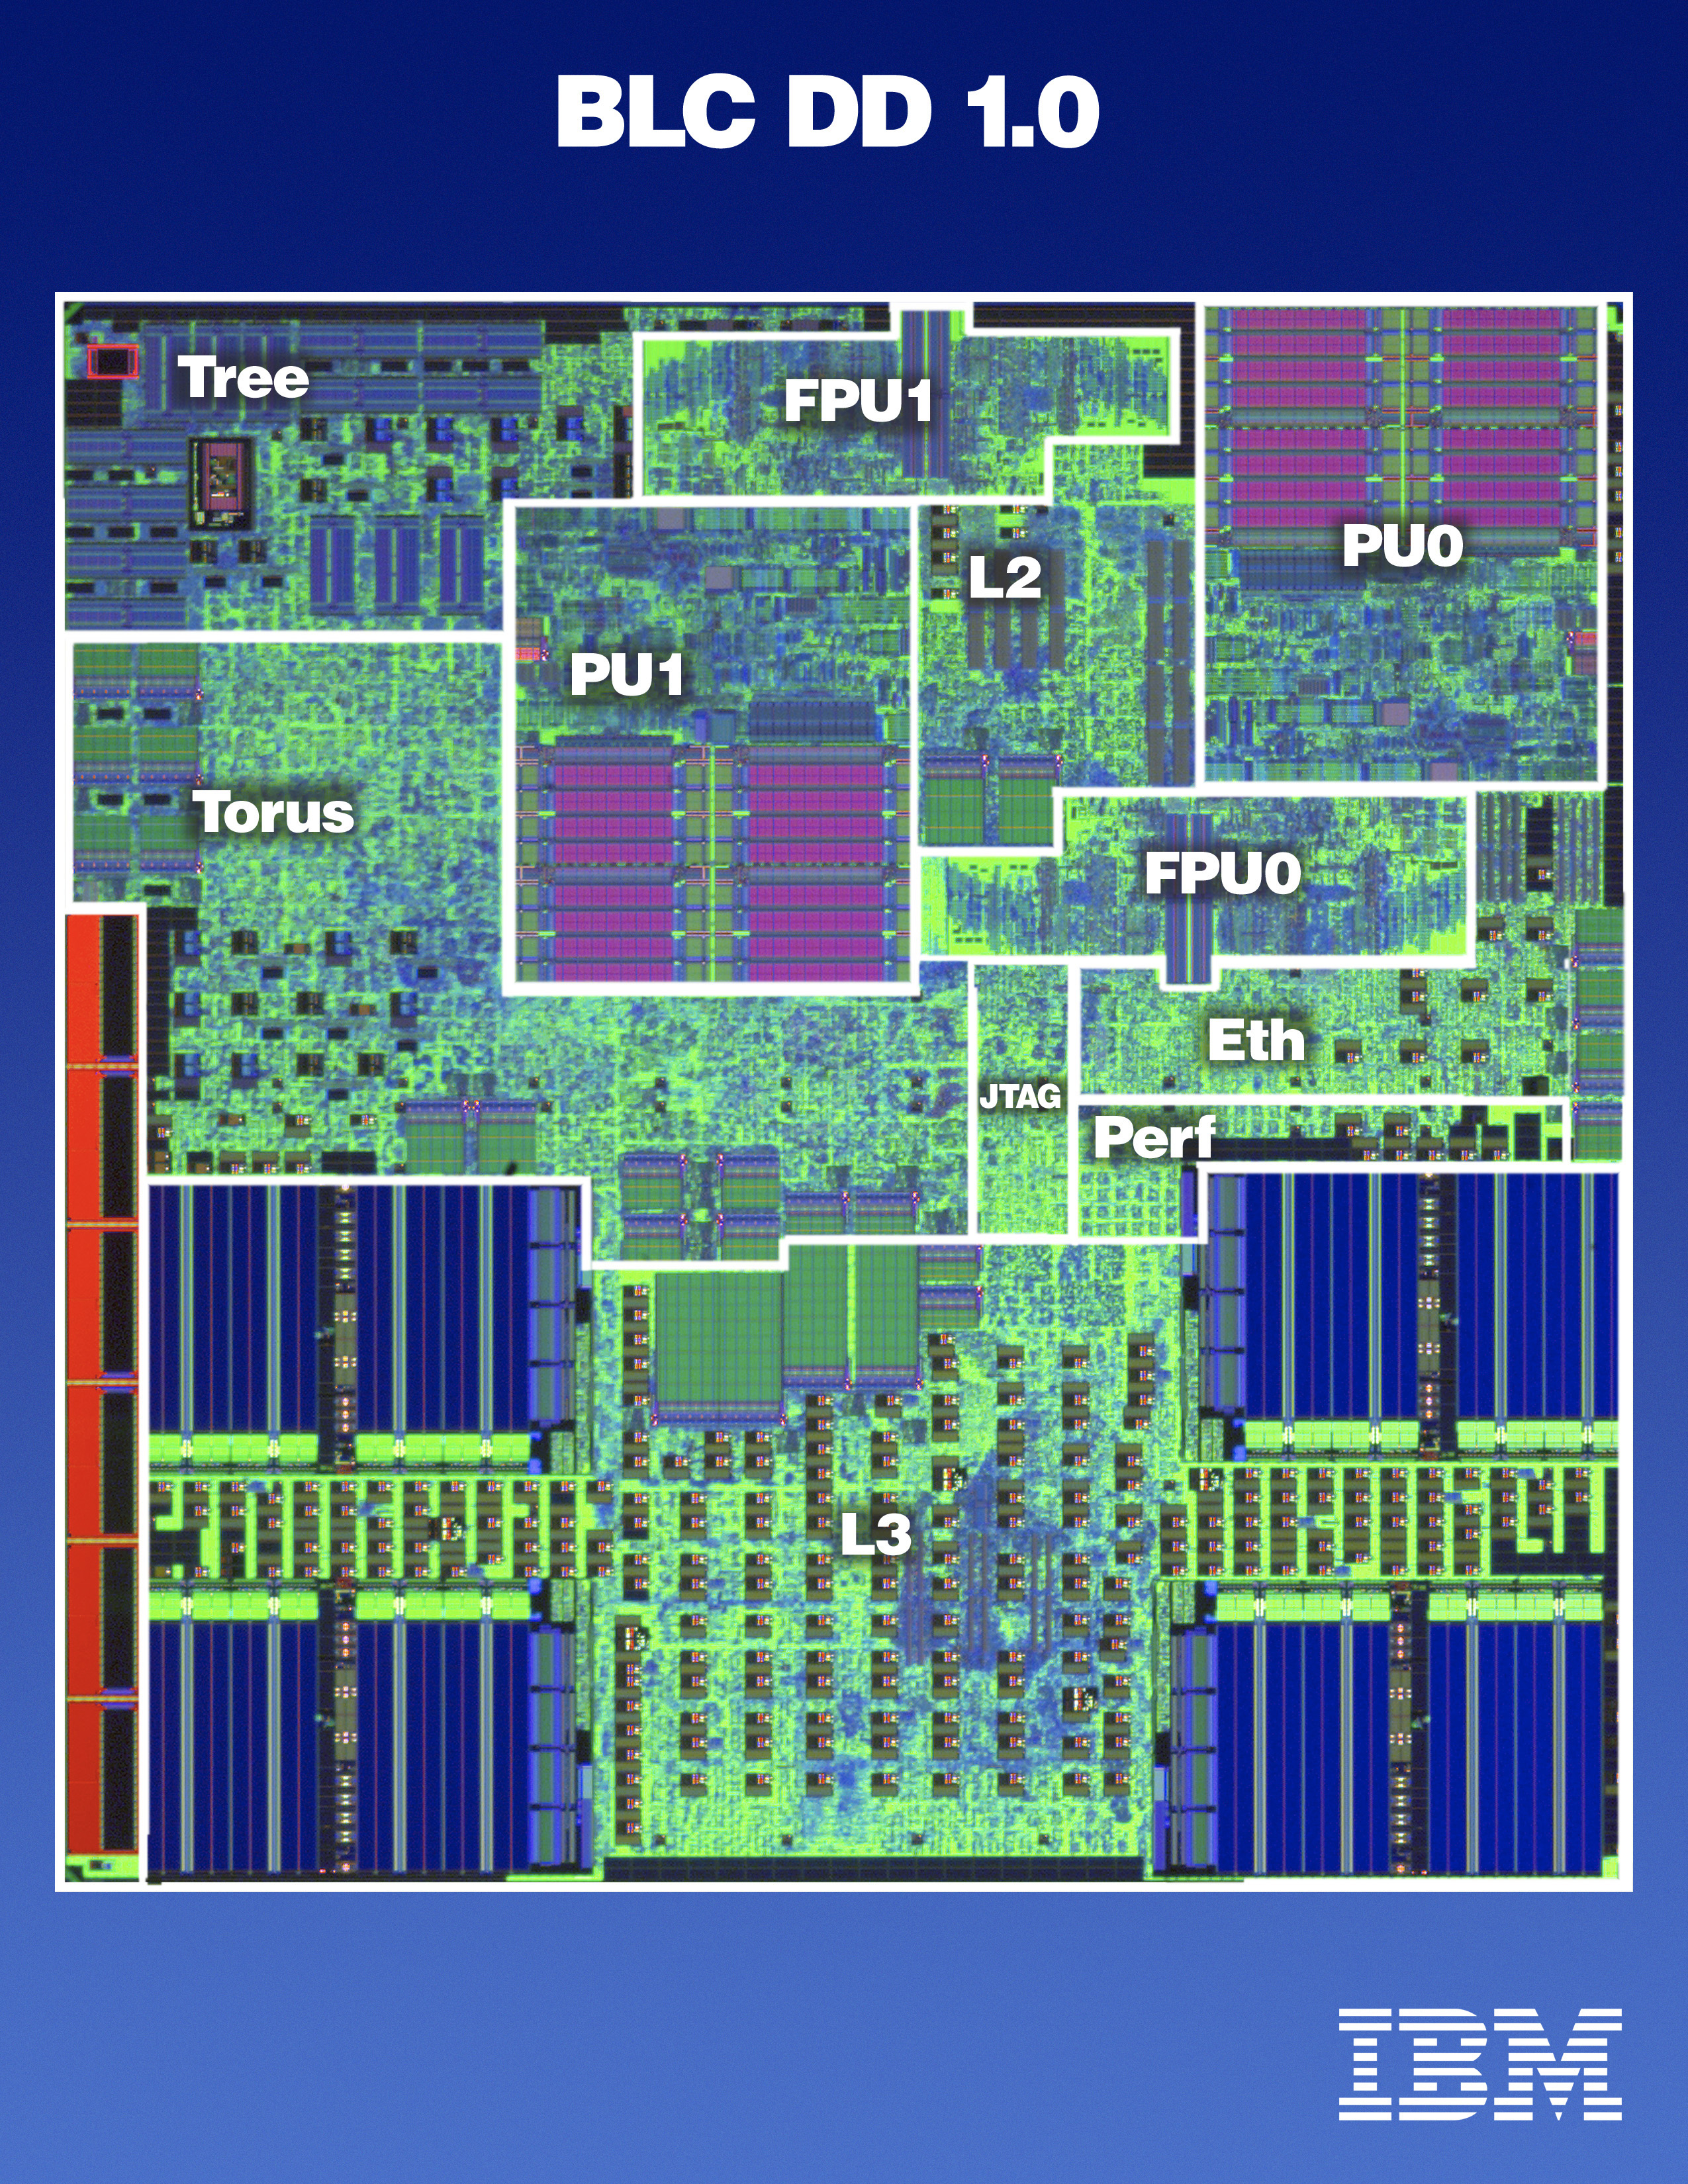
\includegraphics[width=.3\textwidth]{bglchip.eps} 
}
\caption{\label{bglchip}Blue Gene/L CPU showing dedicated network hardware (Torus, Tree, Eth, and JTAG). Note that on most CPUs the Eth block is not connected.}
\end{figure}

The system we are currently using, the Blue Gene/P system at Argonne National Labs, has 40,000 Power PC 450 CPUs, 
with four cores and 2 Gbytes of memory each (for a total of 80 TB of memory). The memory is not globally addressable; communications are entirely via message passing. 
There are two CPU classes, I/O and Compute. What distinguishes the two types is their network connectivity. I/O nodes connect
to three networks: a 10 Gbit/second Ethernet, a 2.4 Gbit/second collective network which has a tree-like topology, and
a JTAG network for control and booting. The Compute nodes are attached to a 3D toroidal mesh network with six links per compute node and 500 MBytes/second bandwidth on each link.  The compute nodes are also connected to the collective, or {\em tree}, network, and the JTAG network. The only connection between CPU nodes and I/O nodes is the tree network. The tree network is used for both computation support (CPU nodes only) and I/O (CPU node to I/O node communications). The I/O nodes, as the name implies, perform file system I/O as proxies for the 
compute nodes. For further detail the reader is referred to \cite{plan9bgp}. 

Currently, Blue Gene systems run two different kernels. The I/O nodes run Linux. The compute nodes run a lightweight kernel, the Compute Node Kernel or CNK. The CNK does not support file I/O directly; instead, system calls are packaged and forwarded to the I/O node. Experimentation with running Linux on the compute nodes is ongoing. 

\subsection{Plan~9}
Plan~9\cite{Plan9} is a distributed operating system developed at Bell Labs. In Plan~9, the only components hardwired into the kernel are those which are absolutely necessary for basic operations (drivers); other components, which can be on the same or other computer, are run outside the kernel (servers). Drivers include hardware controllers, process management, and network protocol stacks. Servers include traditional functions such as file systems and nontraditional functions such as window managers and Grid management tools. Drivers and servers can be transparently intermixed and their locations are 
irrelevant; a server can be reimplemented as a driver with little if any code modification (the TCP/IP stack was originally a server but was moved into the kernel as a driver). For the purposes of this paper, one can consider Plan~9 to be a Unix-like operating 
system with a more compact code base than Unix systems, since a great deal of functionality is provided by user-level services, not kernel services. As mentioned, all file servers are external to the kernel; even the 
RAMdisk 
device is implemented with a user-level process. 


\section{Blue Gene networks and the OS Bypass question}
An early Blue Gene design decision was that  compute node applications would have direct user access to most network interfaces, i.e., the operating system would play no role whatsoever in moving data from program to program. This 
design follows HPC practice of the last 20 years, in which it is taken as a given that the operating system 
is incapable of supporting the networking demands of applications, and the application must "go around" the operating system and drive the network itself. This model, called OS bypass, is a software technique in which the application, not the operating system 
kernel, controls the network interface, managing details including DMA and interrupts. 
We show a simplified version of the normal path in Figure \ref{ospath}, and an OS Bypass example in Figure \ref{osbypass}.
\begin{figure}
\includegraphics[width=2.5in]{ospath}
\caption{\label{ospath}The common OS path for I/O}
\end{figure}
\begin{figure}
\includegraphics[width=2.5in]{osbypass}
\caption{\label{osbypass}An OS Bypass example.}
\end{figure}
The kernel driver is disabled, or, in some cases, removed; the functions of the driver are replaced by 
an application or library. 
All HPC systems in the ``Top 50'', and in fact most HPC systems in the Top 500, use OS bypass. Applications can not 
achieve the needed performance if the operating system is involved in data movement for networking. 

OS Bypass is the network equivalent of what systems such as X Windows do for graphics. 
As the name implies, the OS is completely bypassed; packets move only at the 
direction of the application. OS Bypass involves the application (or libraries) in the
lowest possible level of hardware manipulation, requiring
application libraries to replicate much of the operating systems
capabilities in networking. 

HPC network software performance is frequently characterized in terms of ``bits to the wire'' (BTW) and ``ping-pong latency''. 
Bits to the wire is a measure of how long it takes
from the time an application initiates
network I/O for the bits to appear on the physical wire. Ping-pong latency 
is time it take a program to send a very small packet (ideally, one bit) from 
one node to another, and get a response (usually also a bit). 
These numbers are important as they greatly impact the performance of collectives (such as a global sum), 
and collectives in turn can dominate application performance\cite{petrini}\cite{ 10.1109/HPC.1997.592137}\cite{quadrics}.
In an ideal world, ping-pong latency is four times the "bits to the wire" number. 
Some vendors claim to have hit the magical 1 microsecond ping-pong number, but a more typical 
number is 2-3 microseconds, with a measured BTW number of 700 nanoseconds. 
However, these numbers always require dedicated hosts, devices
controlled by the application directly, no other network activity, 
and very tight polling loops. 

A problem with OS bypass is that the HPC network becomes a single-user device. Because one application 
owns the network, that network becomes unusable to any other program or to the kernel. This exclusivity requires, in turn, that all
HPC systems be provisioned with several networks, increasing cost and decreasing reliability. While the reduction in reliability is not obvious, one must consider 
that the two networks are not redundant; they are both needed for the application
to run. A failure in either network aborts the application.

Our work on Plan~9 for HPC has been to move the communications back into the kernel. The motivation 
for this work follows on measurements of the amount of  code that has been written over the years for OS Bypass layers that recreates the functions of an operating system 
and the difficulty the systems have in making correct decisions about concurrrency, allocation, physical to virtual mappings, and other 
areas that are easy to do in a kernel and very hard to do in a library. As a result the libraries tend to be large and complex: the IBM Deep Computing Messaging Facility for Blue Gene, which is used to support
higher-level libraries such as MPI, is 81,000 lines, as compared to 64,000 lines for the entire Plan~9 kernel  for BG/P (as measured by David Wheeler's sloccount). 

By providing the network to programs as a kernel device, rather than a set of raw registers, we are making HPC usable 
to more than just specialized programs. For instance, the global barrier on the Blue Gene systems is normally only 
available to programs that link in the Deep Computing Messaging Facility (DCMF) library or the 
MPI libraries\footnote{MPI libraries are typically much larger than the Plan~9 kernel; indeed, the configure script for OpenMPI is larger than the Plan~9 kernel}, which in turn 
link in the DCMF. Any program which wishes to use the HPC network must be written as an MPI 
application. Not all applications can be written as MPI applications. Applications writers must recast their 
programs as MPI programs, even when that is not appropriate, because it is not practical 
to reimplement the entire user-mode driver stack. 
Shells are not MPI applications; it makes
no sense whatsoever to turn the shell into an MPI application, as it has uses outside of MPI, such 
as starting MPI applications! As we showed above, making the networks available as real devices can be very useful. 

One might think that the  drivers, in order to equal the performance of OS bypass, need to impose a very 
low overhead -- in fact, no overhead at all: how can a code path that goes through the kernel possibly equal an
inlined write to a register? The overhead of a user level library can in fact be very high. As mentioned, the DCMF library is larger than Plan~9; the 
MPI library is still larger. The measured time to get a packet through these layers is from 2 to 5 microseconds. The OS has a chance. 

%Hence, while it is true that OS bypass has zero overhead in theory, it can have non-zero overhead in fact. 
%Programs that use OS bypass always use a library; the library is usually threaded, with a full complement of locks (and 
%lockiing bugs and race conditions); OS functions are now in a library. In the end, we have merely to offer lower overhead than the library. 

There are security problems with OS bypass as well. 
To make OS bypass work, the kernel must provide interfaces that to some extent break the security model. On Blue Gene/P, for 
example, DMA engines  are made available to programs  that allow them to overwrite arbitrary parts of memory. On Linux HPC clusters, 
Infiniband and other I/O devices are mapped in with mmap, and users can activate DMAs that can overwrite parts of kernel memory. Indeed, 
in spite of the IOMMUs which are supposed to protect memory from badly behaved user programs, 
there have been recent BIOS bugs that allowed users of virtual network interfaces to roam freely over memory above the 4 gigabyte
boundary\cite{iommubug}. Mmap and direct network access are  really  a 
means to an end; the end is low latency bits to the wire, not direct user access. It is so long 
since the community has addressed the real issue that means have become confused with ends. 

\section{Related work}
The most common way to provide low latency device I/O 
to programs is to let the programs take over the device. 
This technique is most commonly used on graphics devices. Graphics devices are inherently single-user devices, with multiplexing 
provided by programs such as the X server. Network interfaces, by contrast, are usually designed with multiple users in mind. 
Direct access requires that the network be dedicated to one program. Multi-program access is simply impossible with 
standard networks. 

Trying to achieve high performance while preserving multiuser access to a device 
has been achieved in only a few ways. In the HPC world, 
the most common is to virtualize the network device, such 
that a single network device appears to be 16 or 32 or more network devices. The device 
requires either a complex hardware design or a microprocessor running a real-time operating system, as in 
Infiniband interfaces: thus, the complex, microprocessor-based interfaces do bypass the main OS, 
but don't bypass the on-card OS\cite{Boden95myrinet}. 
These devices are usually 
used in the context of virtual machines. Device virtualization  requires hardware changes at every level of the system, including
the addition of a so-called iommu\cite{iommu}. 

An older idea is to dynamically generate code as it is needed. For example, the code to read a certain file can 
be generated on the fly, bypassing the layers of software stack. One implementation of this idea 
is found in   Synthesis\cite{synthesis}. While the approach is intriguing, 
it has not proven to be practical, and the system itself was not widely used. 

The remaining way to achieve higher performance is by rigorous optimization of the kernel. Programmers
create hints to the compiler, in every source file, about the expected behaviour of a branch; locks are removed; 
the compiler flags are endlessly tweaked. In the end, this work results in slightly higher throughput, but the 
latency -- "bits to the wire" -- time changes little if at all. It is still too slow. Recent experiences show that 
very high levels  
of optimization can introduce security holes, as was seen when a version of GCC 
optimized out all pointer comparisons to 
NULL. 

Surprisingly, there appears to have been little other work in the area. The mainline users of operating systems do not care; they consider 1 millisecond 
BTW to be fine. Those who do care use OS bypass. Hence the current lack of 
innovation in the field: the problems are considered to be solved. 

The status quo is unacceptable for a number of reasons. Virtualized device hardware increases costs at every level in the I/O path. Device
virtualization 
adds a great deal of complexity, which results in bugs and security holes that are not easily found. The libraries which use these 
devices have taken on many of the attributes of an operating system, with threading, cache- and page-aligned resource allocation, 
and failure and interrupt management. Multiple applications using multiple virtual network interfaces end up doing the same work, with the same
libraries, resulting in increased memory cost, higher power consumption, and a general waste of resources all around. In the end, the applications 
can not do as good a job as the kernel, as they are not running in privileged mode. Applications and libraries do not have access to
virtual to physical page mappings, for example, and as a result they can not optimize memory layout as the kernel code. 

\section{Our Approach}
Before we explain our approach we will first give a quick overview of file I/O in Plan 9. It is similar to the Unix-compatible OSes such as the various BSDs and Linux, 
but at the same time there are enough differences to make an outline useful. 

Processes perform I/O with only two system calls, read and write, as compared to the plethora used on Unix. As on all Unixes, I/O is initiated by a system call trap. 
The kernel then takes the folowing steps:

\begin{itemize}
\item Validate the system call number.
\item Call the system call function. From this point on we will discuss the write function. 
\item Assemble arguments. Arguments are pulled from the stack, which involves a copyin. Register parameters are used in only a limited way in Plan~9. 
\item validate the fd, convert it into an internal pointer to a channel (i.e. file) struct and increment the usage lock to ensure the channel is not closed while in use. 
\item The virtual address and length are validated. The semantics of write require that the process block 
until the data is completely used, or that the process not be able to change the data once the write call returns (i.e. 
the semantics do not allow asynchrony). Some Unix systems support asynchrony by fiddling with the 
page attribute bits, ensuring that post-system-call changes occur in a different page. Others copy data to an internal buffer. Others block the process until the data is no longer needed. 
In keeping with the goal of simplicity, Plan~9 copies the data or blocks the process. 
\item Indirect through the channel structure members to call the driver write function
\item On return, manage any errors and unlock the channel. 
\item Set up return results
\end{itemize}

In most cases, the steps outside the actual I/O itself are not expensive relative to the actual I/O. If the write involves
sending packets over an Ethernet, or writing a disk, the fd and address validation are insignificant, a few microseconds at most. The picture changes completely with a slow processor (as the PowerPC 450 is) and a fast network, as we have on Blue Gene. Then, the overhead of setting up the arguments alone can dominate the overall time. A global barrier operaion across 65536 nodes can be done in 125 nanoseconds 
on Blue Gene; that is 106 instructions. On these measurements, the cost of I/O is made in 1.2-nanosecond increments, and every one counts. 

As can be seen above, there is a lot of repeated work for each system call. It is reasonable to ask just how much the arguments vary for each write system call. How much of this work is unnecesary because we are validating the same parameters over and over? 
We instrumented the Plan~9 kernel and monitored 
applications using  a trace device\cite{iwp9:tracedevice}. We measured all the I/O performed by all processes over 
a 30 minute interval. We learned that, in general, programs read and write a small 
set of files over and over, from a very small set of virtual addresses, with a very limited and small range of sizes. This result makes intuitive sense: consider programs on Unix which use stdio, for example: file I/O is performed 
to an internal buffer which does not change, and the buffer size is usually limited to a page size or smaller. Other I/O addresses are almost always from the stack (i.e. an auto variable). Our measurements confirm this intuition, at least for Plan~9. 

We learned that the bulk of the time for basic device I/O with very small write sizes -- the type of operation common to collective operations -- was taken up in two functions: the one that validated an open file descriptor, and the one that validated an I/O address. 
The measurements indicate that we could benefit from caching active file descriptors and virtual address ranges in each process structure. Caching virtual to real translation information for just 32 address ranges would eliminate all page table walks for almost all process I/O. Caching just 8 file descriptors would eliminate almost all file descriptor validation operations. Of course, this caching would not cover some extreme cases (Apache), but it would cover the most common. 

%The basic I/O path and opportunities for caching are shown in Figure \ref{caching}.
%\begin{figure}
%\caption{\label{caching}Plan~9 I/O path and caching opportunities
%\end{figure}

At the same time, such caching adds a level of complexity that is not consonant with the structure of the Plan~9 kernel. Caches must be validated and cleaned. There would be interactions with other processes and the virtual memory subsystem. Callbacks would be needed when a process forked or exited to make sure cached file descriptors are managed. 

While we considered the caching approach, we eventually rejected it for two reasons. The first was the complexity and the opportunity for introducing bugs. The second was that it might increase the amount of code being run, or at the least not decrease it enough. What we need is a system call interface that eliminates almost all of the kernel code save the actual driver I/O steps -- we want to do a type of OS bypass, but after the OS has been entered. What we want is to bypass all the generic system call code and get right to the business of performing actual I/O. 

Our approach is a modification of the Synthesis approach. We do create curried functions with optimized I/O paths, 
\begin{figure}
\includegraphics[width=2.5in]{curry}
\caption{\label{curry}Our approach: in-kernel OS Bypass}
\end{figure}
but we do not generate code on the fly; curried functions are written ahead of time and compiled with the kernel, and only for some drivers, not all. The decision 
on whether to provide curried functions is determined by the driver writer. 
This approach can be thought of as an {\em in-kernel OS Bypass}. While programs must still switch to the OS to do the I/O, much of the standard OS processing is bypassed, since it is done ahead of time. 

At run time, if access to the curried function is requested by a program, 
the driver  pre-evaluates and pre-validates arguments and sets up the parameters for the driver-provided curried function. 
Commands are written to the {\tt ctl} file of the driver to set up the fast path. 
The 
curried function is made available to the user program as a private system call, i.e. the process structure for 
that one program is extended to hold the new system call number and parameters for the system call. 
Thus, instead of actually synthesizing code at runtime, we augment the process structure so as to 
connect individual user processes to curried 
functions which are already written, with a customized set of parameters contained in a struct attached to the proc structure. 

We have achieved sub-microsecond system call performance with these two changes. The impact of the 
changes on the kernel code is quite minor. 

We will first digress into the nature of Curry functions, describe our changes to the kernel and, finally discuss the 
performance improvements we have seen. 

\subsection{Currying}
The technique we are using, Currying, is well known in mathematical circles. 
We will illustrate it by an example. 

Given a function of two variables, $ f\left( x, y\right) = y/x$, 
one may create a new function, $g\left( x\right)$, 
if $y$ is known,  such that $g\left( x\right) = f\left( x, y\right)$. 
For example, if y is known to be 2, the function g might be $g\left( x\right) = f\left( x, 2\right)$. 

We were interested in applying this idea to two key system calls: read and write. Each takes a 
file descriptor, a pointer, a length, and an offset. 

The application of currying was obvious: given a program which is calling a kernel function read or write function: $ f\left( fd, address, size\right) $, with 
the same file descriptor and same address, we ought to be able to make a new function: 
$g\left( size\right) = f\left( fd, address, size\right)$, or even 
$g\left( \right) = f\left( fd, address, size\right)$. 

Tracing indicated that we could greatly reduce the overhead. Even on an 800 Mhz. Power PC, we could 
potentially get to 700 nanoseconds. This compares very favorably with the 125 ns it takes the hardware to actually
perform the global barrier (that time is included in the 700 ns.).

\subsection{Connecting curry support to user processes}
The integration of curried code into the kernel is a problem. 
Dynamic code generation looks more like a security
hole than a solution. 

Instead, we extended the kernel in a few key ways: 
\begin{itemize}
\item extend the process structure to contain a private system call array, used for fastpath system calls
\item extend the system call code to use the private system call array when it is passed an out-of-range system 
call number
\item extend the driver to accept a fastpath command, with parameters, and to create the curried system call
\item extend the driver to provide the curried function. The function uses only pre-validated arguments from the private system call entry structure
\end{itemize}

\section{Implementation of private system calls on Plan~9 BG/P}
To test the potential speeds of using private system calls, a system was implemented to allow fast writes to the barrier network, specifically for global OR operations, which are provided through {\tt /dev/gib0intr}. The barrier network is particularly attractive due to its extreme simplicity: the write for a global OR requires that we write to a 
Device Control Register, a single instruction, which in turn controls a
wire connected to the CPU. Thus, it was easy to implement an optimized path to the write on a per-process basis.

The data structure for holding pre-validated arguments is shown in Figure \ref{scstruct}. Note that this structure can be very simple, as there are only two I/O calls in Plan~9. 

\begin{figure}
\begin{verbatim}
struct Fastcall {
        /* System call number */
        int	scnum;
        /* File */
        Chan*	c;
        /* Function */
        void	(*fun)(Ar0*, Fastcall *);
        /* Pre-validated arguments */
        void*	buf;
        int	n;
        vlong	offset;
};
\end{verbatim}
\caption{\label{scstruct}Fast system call struct}
\end{figure}

To set up the private system call, programs are required to provide a system call number, a file descriptor, pointer, and length.

Next, we modified the Blue~Gene barrier device, to accept {\tt fastwrite} as a command when written to {\tt /dev/gib0ctl}. When the command is written, the kernel allocates a new {\tt Fastcall} and attaches it to the proc structure. The code to set up the fast path is shown in Figure \ref{code}.
\begin{figure}
\begin{verbatim}
int cfd, gdf, scnum=256;
char area[1], cmd[256];
gfd = open("/dev/gib", ORDWR);
cfd = open("/dev/gib0ctl", OWRITE);
cmd = smprint(
  "fastwrite %d %d 0x%p %d", 
  scnum, fd, area, sizeof(area));
write(cfd, cmd, strlen(cmd));
close(cfd);
docall(scnum);
\end{verbatim}
\caption{\label{code}Sample code to set up a fastpath systemcall}
\end{figure}

Following the {\tt write}, {\tt scnum} contains a number for a private system call to write to the barrier network. From there, a simple assembly function (here called {\tt docall}) may be used to perform the actual private system call. The code is shown in Figure \ref{docall}. 

\begin{figure}
\begin{verbatim}
TEXT docall(SB), 1, $0
    SYSCALL
    RETURN
\end{verbatim}
\caption{\label{docall}User-defined system call code for Power PC}
\end{figure}

When a system call interrupt is generated, the kernel typically checks if the system call number matches one of the standard calls; if there is a match, it calls the appropriate handler, otherwise it gives an error. However, the kernel now also checks the user process's private system call set and calls the fast path function call if a matching private call exists. In the case of the barrier device, it calls {\tt gibfastwrite}, which writes '1' to the Device Control Register. The fastcall avoids several layers of generic code and argument checking, allowing for a far faster write.

\subsection{A non-general-purpose specialization}
The modifications described in the previous section can be considered as general purpose, in the sense 
that any device can be extended to take advantage of them. We have even created Curried pipes. 

In this section we consider specializations that are very specific to the Blue Gene Torus. These specializations extend the kernel in non-general ways, to accomodate an interface that is key to the performance of the machine. The extensions are inspired by Active Messages\cite{von1992active},  and tailored to the needs of a graph application. 

\subsubsection{The Graph Application: motivating intrusive changes}

Graph search on a massive scale (trillions of nodes)
is an important problem in computing. 
Processing   large  graphs   is  becoming   increasingly  important
for  many domains such as social networks and bioinformatics. 
In a graph data structure,
relationships are stored using vertices and edges; a vertex
may represent an object or concept, and the relationships between them
are represented by edges.  The power of graph data structures lies in
the ability to encode complex relationships between data and provide a
framework to analyze the impact of the relationships.

Unfortunately, many algorithms and implementations do not
scale with increasing  graph sizes.  Graph search  places difficult requirements on HPC systems, such that in many cases
programmers are reluctant to run it on anything but a shared-memory machine. 
From the point of view of these applications, even the overhead of an MPI send is so high that the programmers write complex 
queue software that batches small messages into larger ones: the programmers implement queues to reduce the overhead of the many
queues hidden in the stacked layers  of communications libraries and hardware. There is a performance cost to stacked abstractions. 

In contrast to using a  more globally synchronous MPI-based
approach to this problem, we advocate an asynchronous approach for graph analysis\cite{Pearce2010}
and are building messaging infrastructure to accommodate the needs
of applications requiring lightweight asynchronous messaging.
Recently, a challenging graph processing benchmark has been released,
The Graph500 \cite{Graph500}, which involves computing a Breadth-First
Search on massive scale-free graphs.

Two useful programming constructs for this applications are a very fast send for short messages, and a shared-memory ring for received
messages. In all cases, the messages are less than 100 bytes. 
Because the hardware implements a shared-memory ring, it is not necessary to implement the rings 3 times at 3 levels in software for the send side. On the receive side, the hardware also 
implements a shared-memory ring, but it is important to dequeue messages from this ring as quickly as possible; the delivery rate of messages might not match well to the consumption rate of the 
algorithm, and a receive-side overrun is not easy to recover from on the Torus. The interface we present to the user is a function which transmits one short message at a time; and which 
provides the programmer with a function that dequeues messages from a shared-memory ring into an array of messages. The library is called amring, for Active Message Rings. 

In Figure \ref{amringexample} we show a usage of the interface for the common ``MPI Ring'' benchmark. The library provides {\tt myrank} and {\tt nrank}, indicating a processes
rank and the total number of ranks respectively. For local setup, the  {\tt amrsetup} functions is used 
in this example  to set up a 1 Mbyte ring.  The amring structure returned by amrsetup is used in all subsequent operations. 
For global setup, the {\tt amrstartup} function performs a global reduction to make sure all 
programs are running and the Torus is configured for amrings. The {\tt amrsend} and {\tt amrrecv} runctions send and receive, 
respectively. 

In this example, a packet is relayed from node to node, starting at rank 0 and wrapping back to rank
0. 
Rank 0 starts the rounds with a send, then receives; all other ranks do a 
receive, then send. The program specifies the number of Torus packets to be received in the reference variable {\tt num}; the number
actually received is returned in the reference variable.

\begin{figure*}
\begin{verbatim}
        extern int myrank, nranks;
        int rx[1], ry[1], rz[1];
        int num = 1;
        char data[256];
        AmRing *amring;
        amring = amrsetup(1048576);
        amrstartup(amring);
        if (! myrank) {
                amrsend(amring, data, 240, 1);
                amrrecv(amring, &num, data, rx, ry, rz);
        }  else {
                amrrecv(amring, &num, data, rx, ry, rz);
                amrsend(amring, data, 240, (myring+1)%nranks);
        }
\end{verbatim}
\caption{\label{amringexample}Using Active Messsages Rings for ``MPI Ring'' example}
\end{figure*}

\subsubsection{Amring implementation}
The setup function {\tt amrsetup} is little more than a malloc followed by a 
control operation on the Torus driver switching it amring mode. The {\tt amrstartup} 
function is a global reduce, to make sure all participants have made the switch. The real 
core of the amring library is in the send and receive functions. 

{\tt Amrsend} is implemented via a "system call bypass" mechanism, in which the system call trap code
checks the system call number, and bypasses almost all the system call code to call a low latency 
Torus injection function. We
extended the highly generalized kernel system call code with a very specific bypass for a piece of hardware that only exists on 
one machine. Such an intrusive change makes sense when the stringent requirements of short message 
performance must be accomodated. At the same time, it was fairly easy to implement, requiring changes to only two places in the kernel. 

The receive side data management is more complex and much more far-reaching. Data transfer is performed in an interrupt 
handler in the kernel, requiring a mapping between the user space memory ring and kernel interrupt address space. 
The traditional kernel approach to sharing buffers between kernel and user space is via pinning. Pinning is a complicated 
operation which consumes a great deal of code -- there are almost as many lines of code to support 
pinning in Linux as there are in our entire kernel. 
In our  non-traditional approach, the physical and virtual addresses are the same, and are in addition backed by a 
256 Mbyte page table entry (TLB in PowerPC terms). 
We call this address area the "P=V" space. In our kernel, it is used to back the so-called "BSS", or heap, area of a program. It is implicitly
shared: any references to memory in this part of the virtual address space are backed by the same memory. 

Only a few processes, and usually only one, need to use the P=V space. 
Our kernel limits the use of the P=V space to application processes which are compiled for the
IBM Blue Gene "compute node kernel". These
processes are run using an emulation environment\cite{plan9bgp}, and are set up with the P=V 
space as their heap segment. Standard runtime software such as malloc runs quite normally with this 
special heap, albeit much more quickly due to BSS being backed by 256 MB TLBs. All other programs,
compiled with a standard toolchain, run with non-shared heaps.

The amring ring struct is shown in Figure \ref{ring}. 
\begin{figure}
\begin{verbatim}
struct AmRing {
        /* definitions of sizes
         * These are constant
         */
        unsigned char *base;
        unsigned long size;
        unsigned long logN;
        /* kernel writes,
         * user reads
         */
        unsigned long prod;
        /* pad to cache align */
        unsigned char _116[128-16];
        /* kernel ignores, 
         * user reads/writes
         */
        unsigned long con;
        unsigned char _124[128-4];
};
\end{verbatim}
\caption{\label{ring}Shared memory ring for receive packets.}
\end{figure}
The base is simply a pointer to the base of memory, which consists of a block of 256-byte Torus packets. 
The size and logN are different descriptions of the size, provided in each form for convenience;
 the size must be 256 bytes or more, and always a power of 2. Prod
is the record of bytes produced; con the record of bytes consumed. The padding is done to eliminate any 
chance of false sharing between cores. Both the base and the AmRing struct itself are kept in the P=V 
address space. Hence, user mode, kernel mode, and interrupt handlers can manipulate these structures
with no address translation needed. 

\section{Results for two networks}
\subsection{Global Barrier Network}
We achieved our goal of sub-microsecond bits to the wire. With the traditional write path, it took approximately 3,000 cycles per write. Since the BG/P uses 850 MHz PowerPC processors, this means a normal write takes approximately 3.529 microseconds. However, when using the private system calls, it only takes around 620 cycles to do a write, or 0.729 microseconds. The overall speedup is 4.83. 
The result is a potential ping-pong performance of slightly under 3 microseconds, which is competitive wth the best OS bypass performance. 

\subsection{Torus Network}
The Torus network consists of a 3D toroidal mesh with 6 500 Mbyte/second links. Packets consist of one or more 
256-byte fragments, of which 240 bytes are available for user data. The MPI latency for sending 240  bytes to a remote 
proc is approximately 12.5 microseconds (round trip time is 25 microseconds). The Plan 9 performance was not nearly as good -- the one way time was 25 microseconds. 

We should keep this 25 microseconds in perspective. These are 850 Mhz Power PC RISC CPUs: 
their instruction performance is about that of a high end network card CPU. The send involves several interrupts and scheduling operations, as we are counting remote receive overhead too. The increased time for Plan 9 
to perform this operation is due to the fact that a lot more instructions have to run. 

A set of simple changes to the injection (i.e. transmit) side of the driver shaved 8 microseconds from the total time, 
reducing send overhead from 11 microseconds to 2.8. We did not break the one microsecond barrier in this case, although work continues, but we did get the one way latency to a much more competitive value.

\subsection{Fast system call bypass results on the Torus}
Using the "System call bypass"  fast send, we achieved Torus injection rates of 862 thousand packets/second, or four times the rate of MPI as measured by injection test from the Sandia Messaging Benchmarks\cite{barrett2009application}. 
We measured a packet reception rate, using the same benchmarks, of 
606 thousand packets
per second. 
%\begin{figure}[htbp]
%\begin{center}
%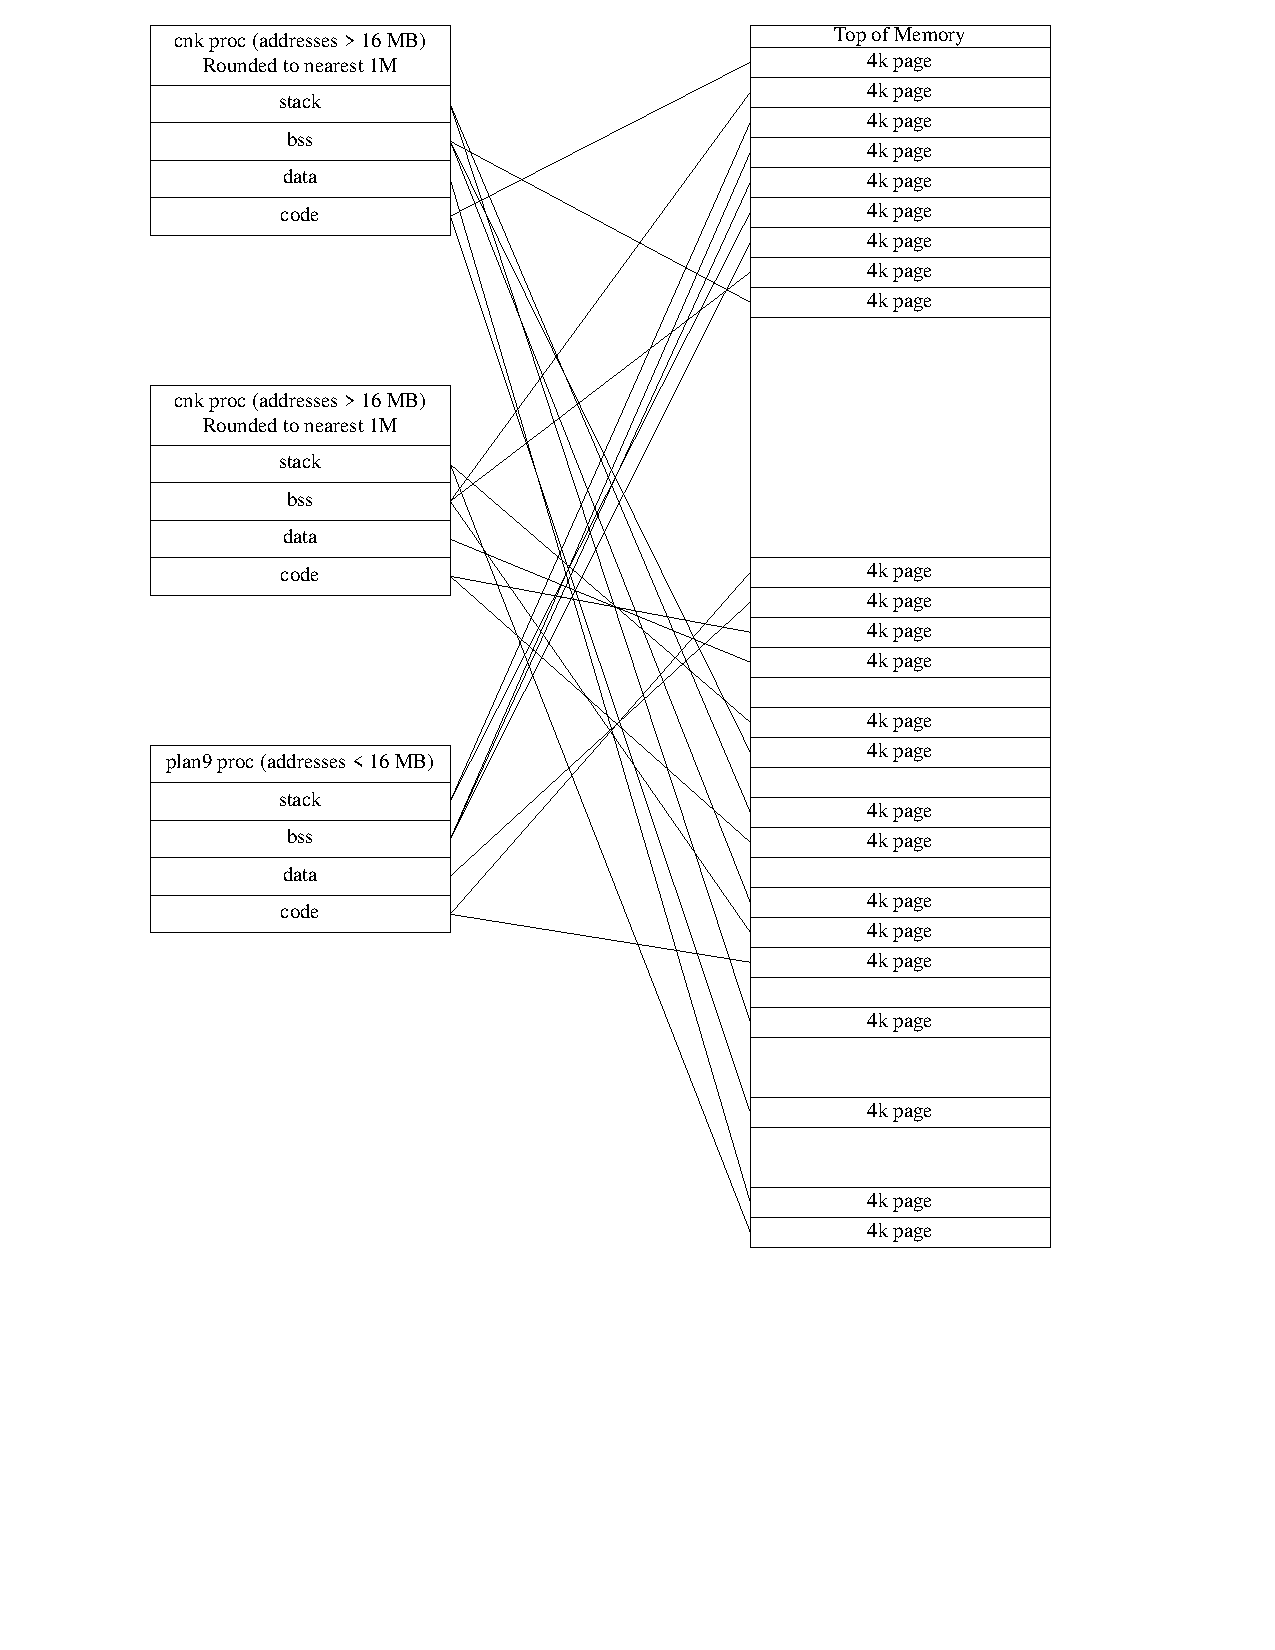
\includegraphics[width=2.5in]{standard}
%\caption{{\bf default}}
%\label{default}
%\end{center}
%\end{figure}

As of this writing we are still working on the graph benchmark. Indications are that it will perform well, but we are exercising a hardware issue which we will have resolved by time of publication. 

\section{Conclusions and Future Work}
The primary function of an operating system is to provide a virtualized set of resources such 
as processors, memory, and the network so that they can be safely shared. 
HPC systems have removed the network responsibility from the operating system for the 
last 20 years. A result has been  the re-creation of OS software above the operating system boundary, including support for device drivers, cache management, memory management, file system protocols, file servers, and many other functions we normally associate with an operating system. 
Only programs written to use the HPC libraries (which include a user-level device driver) 
can make full use of the HPC networks performance\cite{zhang2008design}. 
Still worse, to make the network a multiuser device, operating systems 
functionality is moved into the network interface itself, as in Infiniband interfaces, which provide virtualization at the interface level. 
Frequently, the performance of OS bypass is cited without taking into account the high overhead of these user-level operating systems, and the problems inherent in creating layers of redundant functions between the operating system and programs. 

This paper shows an alternative to the false choice of slow operating systems paths or fast user-level operating systems paths. It is possible to use a general-purpose operating system for I/O and still achieve high performance. While we are not yet equalling the user-level MPI libraries, we are coming from behind, as the user-level libraries and associated network hardware have benefited from 20 years of co-design. 
We wonder what would be possible were the operating system and the hardware designed together, with high performance I/O in mind. 

\section{Acknowledgements}
This work is support by the DOE Office of Advanced Scientific Computing Research. IBM has provided support from 2006 to the present. This research used resources of the Argonne Leadership Computing Facility
 at Argonne National Laboratory, which is supported by the Office of Science
 of the U.S.
 Department of Energy under contract DE-AC02-06CH11357.

\bibliographystyle{plain} 
\bibliography{all}

\end{document}
